\chapter{Normally hyperbolic invariant manifolds}
The objective of this chapter is to extend the theory of low-dimensional stable and unstable manifolds to a general, higher-dimensional setting. The focus will lie on invariant manifolds rather than individual trajectories as invariant manifolds are more observable, more influential, and more robust. We begin with an example.

\begin{ex}[Dynamics near a saddle-type fixed point]
	The difference between the behavior of individual trajectories and of the invariant manifolds is depicted in Fig. \ref{fig:individual_trajectory}. The idea being that under a diffeomorphic transformation of the invariant manifolds of the linear system into those of the nonlinear system, a trajectory starting from a point $x_0$ may be drastically different even if the dynamics remain topologically conjugate to each other. I.e. individual trajectories are sensitive with respect to initial conditions and changes in parameters, meanwhile robust invariant manifolds persist (perturb smoothly).
	\begin{figure}[h!]
		\centering
		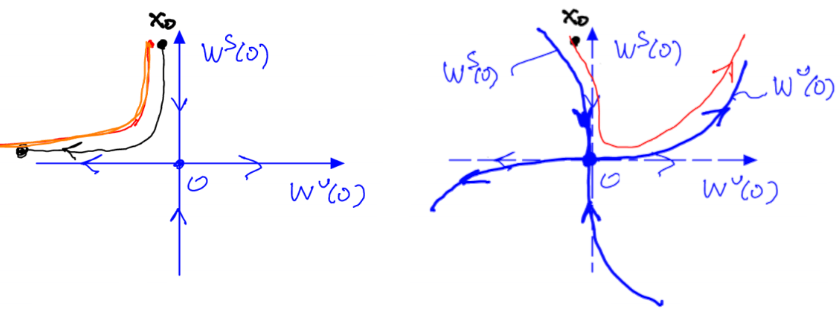
\includegraphics[width=0.6\textwidth]{figures/ch9/1individual_trajectory.png}
		\caption{The dynamics near a saddle-type fixed point demonstrating the sensitive dependence of individual trajectories on initial conditions and changes in parameters, and the robust nature of invariant manifolds.}
		\label{fig:individual_trajectory}
	\end{figure}
\end{ex}

Thus our examination now turns to determining which invariant manifolds are persistent. In order to understand this, first an intermezzo in differentiable manifolds is necessary.

\section{Intermezzo: differentiable manifolds}
\begin{definition}
	A set $M\subset \mathbb{R}^{n}$ is a \emph{$k$-dimensional differentiable manifold}, if it is \underline{locally} diffeomorphic to $\mathbb{R}^{k}$, i.e. for every $x\in M$ there exists an open (in $M$) neighborhood $V\subset M $, such that $V$ is diffeomorphic to an open set $U \subset \mathbb{R}^{k}$. The diffeomorphism between is called the \emph{local parameterization} as is denoted $\Phi:U \to V$. Its smooth inverse is the \emph{local coordinate system} $\Phi^{-1}:V \to U$. These are illustrated in Fig. \ref{fig:diffble_mfd}.
	\begin{figure}[h!]
		\centering
		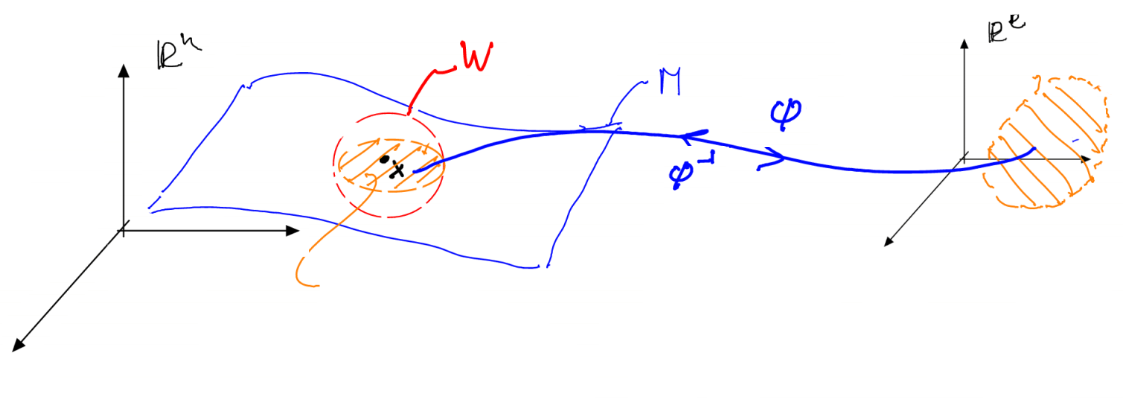
\includegraphics[width=0.7\textwidth]{figures/ch9/2diffble_mfd.png}
		\caption{The differentiable manifold $M$ is given in blue in the left. The red sphere is an open ball in  $\mathbb{R}^{n}$, intersecting this with $M$ yields and open (in $M$) neighborhood $V$ of $ $. The smooth diffeomorphism $\Phi $ transforms $U$ into the open set $U$ of $\mathbb{R}^{k}$.}
		\label{fig:diffble_mfd}
	\end{figure}
\end{definition}

The intuitive meaning of a $k$-dimensional manifold is a $k$-dimensional manifold which locally looks like $\mathbb{R}^{k}$.

\begin{ex}[The circle is a 1-dimensional manifold]
	The circle $\mathcal{S}^{1}$ is a 1-dimensional differentiable manifold. To see define the four open subsets $V_i$ of $\mathcal{S}^{1}$ as open semicircles which are each shifted by $\frac{i \pi }{2} $. Then $\mathcal{S}^{1} = \bigcup_{i=1}^{4}V_i$. These are drawn in Fig. \ref{fig:s1_subsets}. Any $x\in \mathcal{S}^{1}$ belongs to at least one of the $V_i$ due to the previous equality. Furthermore each $V_i$ is diffeomorphic to $U=(-1,1)$ which is open in $\mathbb{R}^{1}$ via the diffeomorphisms
	\begin{subequations}
		\begin{align}
		\Phi_1 &= (t, \sqrt{1-t^2})^{T};&&\Phi_2 = (t, -\sqrt{1-t^2})^{T}; \\
		\Phi_3 &= (-\sqrt{1-t^2}, t)^{T};&&\Phi_4 = (\sqrt{1-t^2}, t)^{T}.
		\end{align}
	\end{subequations}
\begin{figure}[h!]
	\centering
	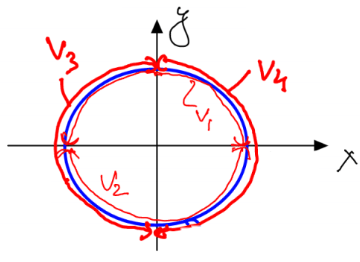
\includegraphics[width=0.3\textwidth]{figures/ch9/3s1_subsets.png}
	\caption{The subsets $V_i$ of $\mathcal{S}^{1} $ which are used to show that the circle is a 1-dimensional manifold.}
	\label{fig:s1_subsets}
\end{figure}

There is no global parameterization of $\mathcal{S}^{1}$, but this is not needed to be a differentiable manifold, and these local parameterizations suffice.	
\end{ex}

\begin{ex}[Not all sets are manifolds]
	A few examples of sets which are not manifolds and the reason as to why not will be given.
	\begin{enumerate}
		\item The figure-eight is not a manifold, as for any point except the central intersection, there exists a local neighborhood diffeomorphic to $\mathbb{R}^{1}$, however at this central intersection, no open neighborhood exists which is diffeomorphic to $\mathbb{R}^{1}$. This is depicted in Fig. \ref{fig:figure_eight}.
			\begin{figure}[h!]
				\centering
				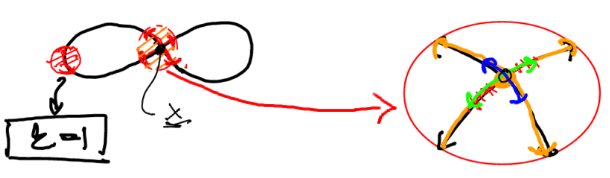
\includegraphics[width=0.5\textwidth]{figures/ch9/3b_figure_eight.png}
				\caption{The figure-eight with the critical intersection which prevents it from being a manifold.}
				\label{fig:figure_eight}
			\end{figure}
		\item A dense orbit on a 2-dimensional torus is not a manifold, as around any point infinitely many adjacent trajectories exist, but do not form a plane (there is a distance between two instances of the trajectory). Hence any neighborhood around any point cannot be hyperbolic to $\mathbb{R}^{2}$ or $\mathbb{R}^{1}$. Such a neighborhood is illustrated in Fig. \ref{fig:dense_orbit_mfd}.
			\begin{figure}[h!]
				\centering
				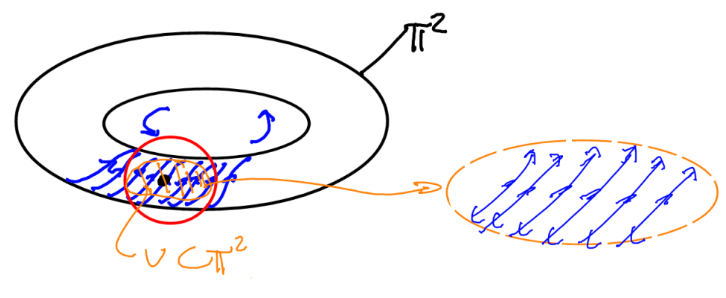
\includegraphics[width=0.5\textwidth]{figures/ch9/4dense_orbits_mfd.png}
				\caption{A depiction of a local neighborhood of a point in a dense orbit of the torus.}
				\label{fig:dense_orbit_mfd}
			\end{figure}
		\item The union of a semi-infinite spiral and semi-open (left closed, right open) interval do not form a differentiable manifold. For this set, at the intersections of the two sets, points with neighborhoods as in the figure eight appear.
	\end{enumerate}
\end{ex}

We can construct manifolds very easily, for instance by taking any smooth function $f:X \to Y$, the graph of $f$ namely the set $ \textrm{graph} (f)=\{(x,y):\ x\in X,\ y=f(x)\}$ is a differentiable manifold. 

\begin{definition}
	For two manifolds $X$ and $Z$, each subsets of $\mathbb{R}^{n}$, with $X \subset Z$ we call $X$ a \emph{submanifold} of $Z$. 
\end{definition}
An example of a submanifold would be $X=\mathcal{S}^{1}\subset Z = \mathcal{S}^{2} \subset \mathbb{R}^{3}$. We say $\mathcal{S}^{1}$ is a 1-dimensional submanifold of the 2 dimension manifold $Z$.

\begin{definition}
	A manifold $M\subset \mathbb{R}^{n}$ is a \emph{$k$-dimensional manifold with boundary}, if it is locally diffeomorphic to a relatively open set in the non-negative half-space $H^{k}\subset \mathbb{R}^{k}$. The \emph{boundary of $M$}, denoted $\partial M$ is always mapped into $\partial H^{k}$ under any parameterization, and is a $k-1$-dimensional manifold. Such a manifold and its parameterization are illustrated in Fig. \ref{fig:bndry_mfd_def}.
	\begin{figure}[h!]
		\centering
		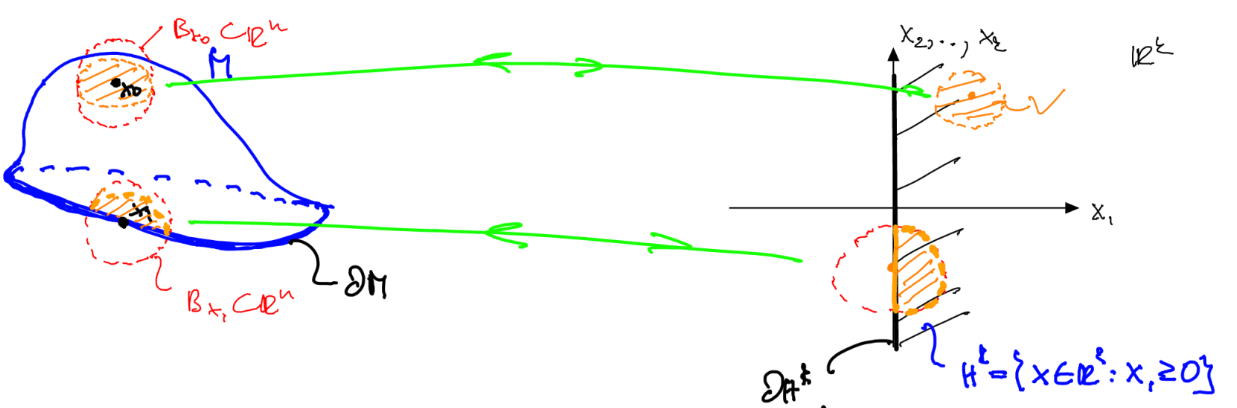
\includegraphics[width=0.7\textwidth]{figures/ch9/5bndry_mfd_def.png}
		\caption{An illustration of the manifold with boundary $M$ and a parameterization mapping its boundary to $\partial H^{k}$.}
		\label{fig:bndry_mfd_def}
	\end{figure}
\end{definition}

Closed intervals, closed cyclinders, and closed hollow spheres are all manifolds with boundaries, however it is not always the case that simply taking the closure of a manifold yields a manifold with boundary. For instance the interior of a rectangle is a manifold (using the identity as a parameterization), however as the corners are not smooth the closure is not a manifold.

\begin{definition}
	Given a manifold $M\subset \mathbb{R}^{n}$ with the local parameterization at $x$ given by $\Phi$ (assume for simplicity that $\Phi(0)=x\in V$), the \emph{tangent space of the manifold} is then defined as
	\begin{align}
		\boxed{
			T_{x}M= \textrm{im} [D\Phi(0)].
		}
	\end{align}
	The intuition as to why this is called the tangent space is show in Fig. \ref{fig:tangent_space_def}.
	\begin{figure}[h!]
		\centering
		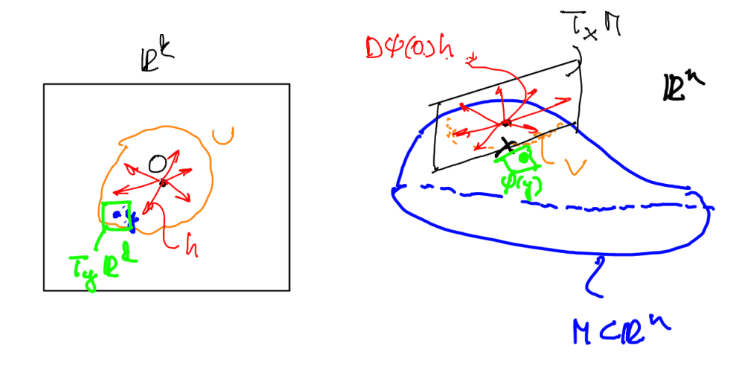
\includegraphics[width=0.65\textwidth]{figures/ch9/6tangent_space_def.png}
		\caption{The tangent space of a manifold $M$. The map $D\Phi(0)$ takes us from the left to the right image, and the map $D\Phi^{-1}(x)$ takes us from right to left.}
		\label{fig:tangent_space_def}
	\end{figure}
\end{definition}

Note here how the differential is defined
\begin{align}
	D \Phi(x)h = \lim_{s \to 0} \frac{\Phi(x + sh) - \Phi(x)}{s}.
\end{align}
Therefore the map $D\Phi(y)$ is a map from the tangent space of $\mathbb{R}^{k}$ at $y$ to the tangent space of $M$ at $\Phi(y)$, i.e. $D\Phi(y): T_{y}\mathbb{R}^{k}\to T\Phi(y)M$. 

\begin{remark}[]
	Note a few facts about tangent spaces:
	\begin{enumerate}
		\item Although it appears that $T_{x}M$ depends on the parameterization $\Phi$, it actually does not;
		\item The dimension of the tangent manifold, which is well defined as it is a linear subspace of $\mathbb{R}^{n}$, is equal to the dimension of $M$, namely $k$;
		\item A map $f:M\to N$ between manifolds induces a linear mapping between the appropriate tangent spaces of the manifolds. Denoting by $\Phi$ and $\Psi$ the respective local parameterizations, the induced map between parameter spaces is $F= \Psi^{-1} \circ f \circ \Phi$. This is a mapping between linear spaces and $DF$ is well-defined. In turn, this implies that $Df$ is well-defined and by the chain rule is equal to $D\Psi \circ DF \circ D\Phi^{-1}$, therefore it is possible to differentiate mappings between manifolds. Then we have the sought-after mapping between tangent spaces 
			\begin{align}
				Df: T_{x}M \to T_{f(x)}N.
			\end{align}
			These maps are illustrated in Fig. \ref{fig:induced_tangent_map}.
			\begin{figure}[h!]
				\centering
				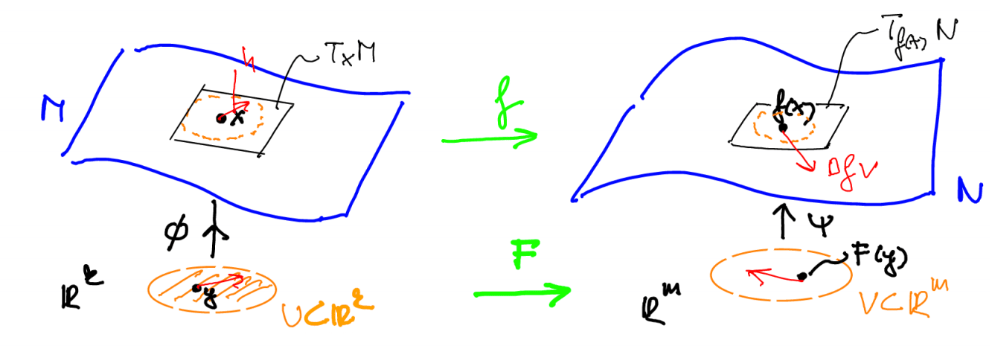
\includegraphics[width=0.7\textwidth]{figures/ch9/7induced_tangent_map.png}
				\caption{The commutative diagram along with the respective spaces illustrated for the induced map between tangent spaces.}
				\label{fig:induced_tangent_map}
			\end{figure}
	\end{enumerate}
\end{remark}

\begin{definition}
	The set of all tangent spaces, labelled by their base points is called the \emph{tangent bundle}
	\begin{align}
		\boxed{
			TM = \left\{ (x,v):\ x\in M,\ v\in T_{x}M \right\} = \bigcup_{x\in M}(x, T_{x}M).
		}
	\end{align}
The tangent bundle is a $2k$-dimensional manifold.	
\end{definition}

By labelling tangent vectors with their respective base points, different tangent spaces are separate \emph{fibers} of the tangent bundle. In general $TM \neq M \times \mathbb{R}^{k}$, i.e. the tangent bundle is not a global direct product. In fact, locally, each tangent bundle is trivial (the direct product), this just does not extend globally. However, for $M=\mathcal{S}^{2}$ the tangent bundle is diffeomorphic to $\mathcal{S}^{2} \times \mathbb{R}^{2}$. 

\begin{definition}
	The \emph{normal space}, unlike the tangent space, depends on the ambient space. For a $k$-dimensional manifold $M$ embedded in $\mathbb{R}^{n}$, the normal space at a point $x$, $N_{x}M$, is the compliment in the direct sum forming the tangent space of the ambient, i.e.
	\begin{align}
		\boxed{
			T_{x}M \oplus N_{x}M = T_{x}\mathbb{R}^{n}.
		}
	\end{align}
	Therefore, the dimensional of the normal space is $n-k$. The normal space is drawn in Fig. \ref{fig:normal_space_def}.	
	\begin{figure}[h!]
		\centering
		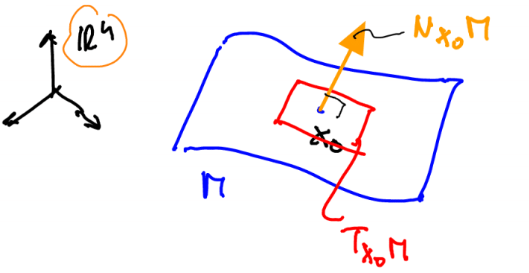
\includegraphics[width=0.45\textwidth]{figures/ch9/8normal_space_def.png}
		\caption{The normal space of a manifold $M$ at the point $x_0$ along with the tangent space at the same point.}
		\label{fig:normal_space_def}
	\end{figure}
\end{definition}

\begin{definition}
	Analog to the tangent bundle, the \emph{normal bundle} is the collection of normal spaces of the manifold $M$ labelled by their base points
	\begin{align}
	\boxed{
		NM = \left\{ (x,v):\ x\in M,\ v\in N_{x}M \right\}.
	}
	\end{align}
\end{definition}
By labelling normal vectors with their base points, intersections are avoided as shown in Fig. \ref{fig:normal_vector_intersection}.
\begin{figure}[h!]
	\centering
	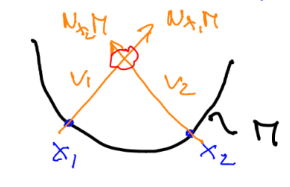
\includegraphics[width=0.3\textwidth]{figures/ch9/9normal_vector_intersection.png}
	\caption{Intersecting normal vectors, these are avoided by labelling vectors with their base points.}
	\label{fig:normal_vector_intersection}
\end{figure}

\begin{definition}
	A \emph{subbundle} of the normal bundle is any $x$-dependent family of subspaces of $N_{x}M$, which is smooth in $x$.
\end{definition}
An example of such a subbundle is given in Fig. \ref{fig:subbundle_ex}, where the smooth family of subspaces is given by $S(x)\subset N_{x}M$.
\begin{figure}[h!]
	\centering
	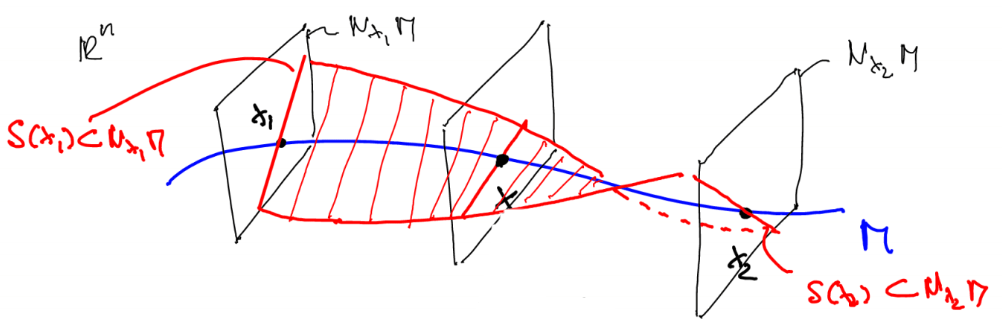
\includegraphics[width=0.8\textwidth]{figures/ch9/10subbundle_ex.png}
	\caption{A subbundle of the manifold $M$, each base point $x\in M$ is a base point of $S(x)$, a fiber of the normal bundle.}
	\label{fig:subbundle_ex}
\end{figure}

\newpage
\section{Theory of normally hyperbolic invariant manifolds}
The framework for the following section will be of a dynamical system
\begin{align}
	\dot{x}=f(x);\quad x \in \mathbb{R}^{n};\quad f\in\mathcal{C}^{r}\ r\geq 1.
\end{align}
Furthermore, let $M_0\subset \mathbb{R}^{n}$ be a $k$-dimensional, compact, $\mathcal{C}^{1}$-manifold with boundary $\partial M_{0}$.

\begin{definition}
	The manifold $M_0$ is an \emph{overflowing invariant manifold} if $f(x)$ points strictly outwards of $\partial M_0$. A special case of this is when $\partial M_0= \emptyset$.
\end{definition}

There are three central questions for what happens to this manifold which we will address:
\begin{enumerate}
	\item Does it persists (survive smoothly)?
	\item Is it stable (what happens to nearby trajectories)?
	\item What is the interior structure of the stable/unstable manifolds of $M_0$?
\end{enumerate}

\begin{ex}[]
	Consider the system
	\begin{align}
		\begin{dcases}
			\dot{x}= -x(1-x)(1+x) \\
			\dot{y} = \alpha y
		\end{dcases}
		;\quad 0 < \alpha \leq 1.
	\end{align}
	Now define $M_0$ to be the closed interval $[-1-\varepsilon, 1 + \varepsilon]\times \{0\}$. This manifold is of dimension 1, has nonempty boundary $\{-1-\varepsilon, 1+\varepsilon\}$, is compact, and smooth. At each point in the boundary, $f$ is pointing away from $M_0$. Therefore, $M_0$ is an overflowing invariant manifold. We also have that $W^{S}_{ \textrm{loc}}(M_0)$ is nonempty, meanwhile $W^{U}_{ \textrm{loc} }(M_0)$ is empty. Trajectories of this dynamical system along with $M_0$ and the stable local manifold are depicted in Fig. \ref{fig:overflowing_mfd_ex1}.
	\begin{figure}[h!]
		\centering
		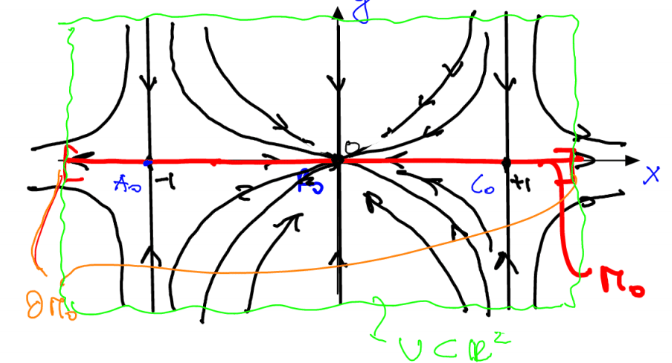
\includegraphics[width=0.6\textwidth]{figures/ch9/11overflowing_mfd_ex1.png}
		\caption{An illustration of the trajectories of the dynamical system, the overflowing invariant manifold $M_0$, its boundary, and the local stable manifold drawn in green. The fixed points $A_0$, $B_0$, and $C_0$ are also shown.}
		\label{fig:overflowing_mfd_ex1}
	\end{figure}

	Now we may ask if $M_0$ is robust under perturbations (if it persists). For example under the perturbation
	\begin{align}
		\begin{dcases}
			\dot{x} = -x(1-x)(1+x) -\varepsilon y \\
			\dot{y} = - \alpha y + \varepsilon x
		\end{dcases}
		;\quad - \leq \varepsilon \ll 1.
	\end{align}
	The fixed points $A_0$, $B_0$, and $C_0$ are hyperbolic, therefore they persist. In fact $B_0$ does not move at all. The other fixed points move to new perturbed counterparts, i.e. $A_0,C_0 \to A_{\varepsilon}, C_{\varepsilon}$. 
	{\color{blue} what is he getting at by defining $y_{\varepsilon} = \frac{\varepsilon}{\alpha}x_{\varepsilon}$ here, not sure how that helps here.}

	At $B_0 = B_{\varepsilon}$ we can linearize to find
	\begin{align}
		\begin{pmatrix}
			\dot{x} \\ \dot{y}
		\end{pmatrix}
		 = 
		 \begin{pmatrix}
			 -1 & - \varepsilon \\
			 \varepsilon & -\alpha 
		 \end{pmatrix}
		 \begin{pmatrix}
		 	x \\ y
		 \end{pmatrix}
		. 
	\end{align}
Depending on $\alpha $ we differentiate two cases.
\begin{enumerate}
	\item $\bm{\alpha =1} $ In this case the eigenvalues split in a vertical fashion, as shown in Fig. \ref{fig:eigv_vertical_split}. {\color{blue} these two look topologically equivalent to me in the figure}.
\end{enumerate}

\end{ex}

The reason for the destruction of the manifold here was the normal rate of attraction being less than or equal to the tangential rate of attraction at one point. This can be exemplified as proceeds.

\begin{ex}[]
	Consider the dynamical system
	\begin{align}
		\begin{dcases}
			\dot{x} = -x(1-x)(1+x) + \varepsilon y \\
			\dot{y} = - \frac{3}{2} y - \varepsilon x
		\end{dcases}
.		
	\end{align}
	This is the specification of the previous example to $\alpha = \frac{3}{2}$. If we linearize at the point $B_0$ for $\varepsilon = 0 $ we find
	\begin{align}
	\begin{dcases}
		\dot{x} = - x \\
		\dot{y} = -\frac{3}{2} y
	\end{dcases}
	.	
	\end{align}
	The solution to the linearized system is
	\begin{align}
		\begin{dcases}
			x(t) = x_0 e^{-t} = x_0 \left(e^{-1} \right)^{t} \\
			y(t) = y_0 e^{-\frac{3}{2}t} = y_0 \left(e^{-\frac{3}{2}}\right)^{t}
		\end{dcases}
		\implies y = y_0 \left(\frac{x}{x_0}\right)^{\frac{3}{2}}.
	\end{align}
	The eigenvalue constellation and linearized phase portrait, along with the implied nonlinear phase portrait for this system are show in Fig. \ref{fig:alpha_specification}.
	\begin{figure}[h!]
		\centering
		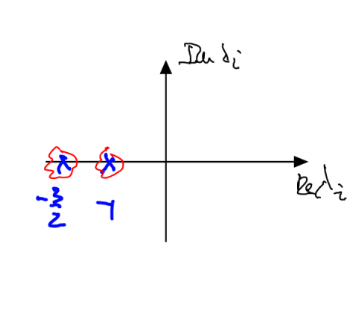
\includegraphics[width=0.27\textwidth]{figures/ch9/12alpha_specification_1.png}
		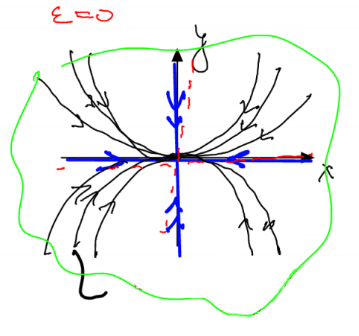
\includegraphics[width=0.27\textwidth]{figures/ch9/12alpha_specification_2.png}
		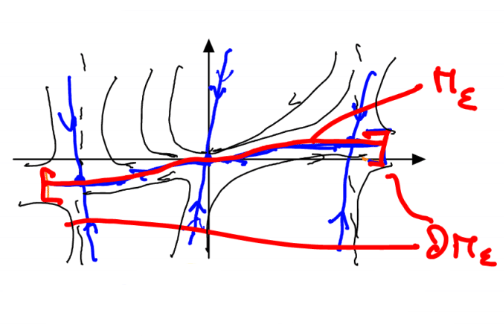
\includegraphics[width=0.4\textwidth]{figures/ch9/12alpha_specification_3.png}
		\caption{Left: The eigenvalue constellation for the linearization around $B_0$ for $\varepsilon=0$. Middle: The linearized phase portrait around $B_0$. Right: The nonlinear phase portrait with the nearby overflowing invariant manifold $M_{\varepsilon}$.}
		\label{fig:alpha_specification}
	\end{figure}
	One can check here that $\dot{y}= (r+\mu )y + \varepsilon x$ would give $\mathcal{C}^{r}$ differentiability for $M_{\varepsilon}$ for $0 \leq \mu \ll 1$. Formally, for $\mu=0 $ we would have $\mathcal{C}^{\infty }$ differentiability, but only for the linear part, and this would not be robust.	
\end{ex}

The general challenge is to quantify the growth/contraction rates in the normal and tangential directions, i.e. how do we determine the rates away from fixed points along trajectories.

Recall our setup with the compact, overflowing invariant $\mathcal{C}^{r}$ manifold $M_0 \subset   \mathbb{R}^{n}$ of dimension $k$, for $r\geq 1$ and the dynamical system 
\begin{align}
	\dot{x} = f(x);\quad x \in \mathbb{R}^{n};\quad f\in \mathcal{C}^{r}.
\end{align}
Now consider the \emph{inverse linearized flow map} on the tangent bundle of $\mathbb{R}^{n}$ for some $t\geq 0$
\begin{align}
	(F^{-t}, DF^{-t}):\ T\mathbb{R}^{n} \to T\mathbb{R}^{n};\ (p,v) \mapsto \left(F^{-t}, DF^{-t}(p)v\right).
\end{align}
This map is depicted in Fig. \ref{fig:inv_lin_flow_map}.
\begin{figure}[h!]
	\centering
	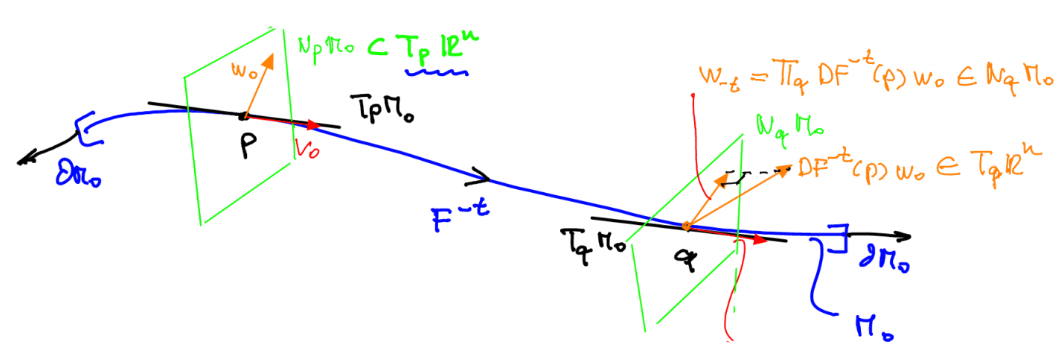
\includegraphics[width=0.95\textwidth]{figures/ch9/13inv_lin_flow_map.png}
	\caption{The inverse linearized flow map. We have $q=F^{-t}(p)\in M_0$ and the red arrow on the right is $v_{-t}=DF^{-t}(p)v_0 \in T_{q}M_0$ for $v_0 \in T_{p}M_0$. The map $\Pi_{q}$ is the orthogonal projection onto $N_{q}M_0$.}
	\label{fig:inv_lin_flow_map}
\end{figure}

To quantify the rate of normal attraction we define for $w_0 \in N_{p}M_0$, as in Fig. \ref{fig:inv_lin_flow_map}, $w_{-t}\in N_{q}M_0$ to be $\Pi_{q}DF^{-t}(p)(p)w_0 $. If we have that
\begin{align}
	\frac{\|w_0 \|}{\| w_{-t}\|}\sim e^{-\alpha t}	= (e^{-\alpha })^{t}; \quad \alpha >0; \quad t \to \infty ,
\end{align}
then the best estimate for such an $e^{-\alpha }$ is 
\begin{align}
	\boxed{
		\nu(p) = \inf \left\{ a \in \mathbb{R}^{+}:\ \lim_{t\to\infty }{\frac{\|w_0\|}{\|w_{-t}\|}}/{a^{t}} = 0,\ \forall w_0 \in N_{p}M_0 \right\}.
	}
\end{align}
The $\inf $ then gives us the smallest upper bound.
{\color{blue} he says largest lower bound, I think this is wrong, the only $a$ which are included in the set we take the inf over are $a$ such that $e^{-\alpha }<a$, i.e. an upper bound. The largest lower bound would be an expression like sup(lim ... = $\infty$) }
The idea behind this, is that for large $a$, the quotient will go to zero {\color{blue} again, this is in line with an upper bound I think}, if we start to lower $a$ until this trend changes we will reach the largest lower 
{\color{blue}smallest upper} bound.

If $e^{-\alpha }=a \sim \nu(p) < 1$ then $M_0$ is exponentially attracting in backwards time. Note that the orbit from $p$ will generally not approach a fixed point. Furthermore, $-\log(\nu(p))$ will generally not be the eigenvalue of a Jacobian (the linearized flow map at a fixed point).

Next, we would like to quantify the relationship between the normal and tangential rates. If we have
\begin{align}
{\frac{\| w_0 \|}{\|w_{-t}\|}}/{\frac{\|v_0\|}{\|v_{-t}\|}} \sim \frac{e^{-\alpha t}}{e^{-\alpha t \cdot \frac{1}{\rho}}}
\end{align}
for some $\rho \in \mathbb{R}$ and $\alpha >0$ as $t\to \infty $ then define the \emph{type number} to be
\begin{align}
	\boxed{
		\sigma(p) = \inf \left\{ b \in \mathbb{R}:\ \lim_{t\to \infty }\left({\frac{\|w_0\|}{\|w_{-t}\|}}/{\frac{\|v_0\|}{\|v_{-t}\|}}\right)^{b} = 0,\ \forall w_0 \in N_{p}M_0,\ \forall v_0 \in T_{p}M_0 \right\}.
	}
\end{align}
The type number is also known as the \emph{Lyapunov-type number} or \emph{Fenichel-type number}. If $\sigma(p) \sim \frac{1}{\rho} < \frac{1}{s}$ for some $s\in \mathbb{Z}^{+}$, then the normal decay to $M_0$ is $s$-times stronger than the tangential compression along $M_0$, at least along the trajectory through $p$.

\begin{remark}[Properties of Fenichel-type numbers]
 First, each are constant along trajectories, and dependent only on the $\alpha $-limit set of the trajectory (the set of limit points as $t \to -\infty $). Also, both $\nu(p)$ and $\nu(p) $ are upper-semicontinuous in $p$ ($\limsup_{p \to p_0} \sigma(p) \leq \sigma(p_0)$).
\end{remark}

Next, it is important to be able to compute the Fenichel-type numbers, to this end define two functions
\begin{align}
	A_{t}(p) &= \left. DF^{-t}(p) \right|_{T_{p}M_0}:\ T_{p}M_0 \to T_{q}M_0;\ q = F^{-t}(p); \\
	B_{t}(p) &= \left. \Pi_{p}DF^{t}(F^{-t}(p)) \right|_{N_{F^{-t}(p)}M_0}:\ N_{F^{-t}(p)}M_0 \to N_{p}M_0.
\end{align}
The reason for the $F^{-t}(p)$ being the inner argument for $B_{t}$ is that we need to step back in order to safely evaluate the linearized map in forward time. With these functions in hand we can calculate the Fenichel-type numbers equipped with the next theorem.

\begin{theorem}[Fenichel (1971)]
We have that the following holds
\begin{align}
	\boxed{\nu(p) = \limsup_{t\to \infty }\| B_{t}(p)\|^{\frac{1}{t}}; }
\end{align}
and if $\nu(p)<1$, then
\begin{align}
	\boxed{\sigma(p) = \limsup_{t\to \infty }\frac{\log\left( \| A_{t}(p) \| \right)}{-\log \left( \| B_{t}(p) \| \right)}.}
\end{align}
\end{theorem}

\begin{ex}[]
	Consider the dynamical system
	\begin{align}
		\begin{dcases}
			\dot{x} = -x(1-x)(1+x) \\
			\dot{y} = -by
		\end{dcases}
		;\quad b>0.
	\end{align}
	Further, define $M_0 = \left\{ (x,y):\ x\in \left[ -\frac{3}{2}, \frac{3}{2}\right],\ y=0 \right\}$. Using the previous theorem, it is possible to show
	\begin{align}
		\nu (A_0) = \nu (C_0) = e^{-b}; \quad \sigma(A_0) = \sigma(C_0) = - \frac{2}{b}; \quad
		\nu (B_0) = e^{-b}; \quad \sigma(B_0) = \frac{1}{b}.
	\end{align}
	The points $A_0$, $B_0$, and $C_0$ along with the manifold $M_0$ are illustrated in the phase space in Fig. \ref{fig:fenichel_ex1}.
	\begin{figure}[h!]
		\centering
		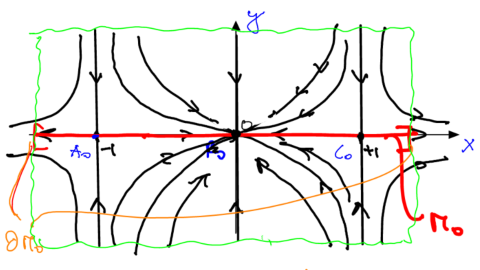
\includegraphics[width=0.5\textwidth]{figures/ch9/14fenichel_ex1.png}
		\caption{$A_0$, $B_0$, and $C_0$ along with the manifold $M_0$ are illustrated in the phase space.}
		\label{fig:fenichel_ex1}
	\end{figure}
\end{ex}

\begin{definition}
	The manifold $M_0$ is an \emph{$r$-normally hyperbolic invariant manifold} if
	\begin{enumerate}
		\item $\nu (p)<1$ for all $p\in M_0$ ;
		\item $\sigma(p) < \frac{1}{r}$ for all $p \in M_0$.
	\end{enumerate}	
\end{definition}
\begin{remark}[]
	If there is no tangential compression, then $\sigma(p)<0$ and $(ii)$ holds automatically for all $r$.
\end{remark}

Building on the previous results, we have the next the next result.
\begin{theorem}[Fenichel (1971)]
Assume we have
\begin{align}
	\dot{x}= f_{ \textrm{pert} }(x) = f_{0}(x) + \Delta f(x);\quad f_0, \Delta f \in \mathcal{C}^{r},\ r\geq 1,
\end{align}
for a compact, overflowing invariant (under $f_0(x)$) manifold $M_0$ which is $\mathcal{C}^{r}$ and $r$-normally hyperbolic. Then for $\|\Delta f \|_{\mathcal{C}^{1}}$ small enough, there exists an overflowing invariant manifold $\tilde{M}_0$ for $\dot{x}=f_{ \textrm{pert} }(x)$, such that
\begin{enumerate}
	\item $\tilde{M}_{0}$ is $\mathcal{C}^{1}$-close to $M_0$ and $\mathcal{C}^{r}$-diffeomorphic to $M_0$ ;
	\item All close enough trajectories converge to $\tilde{M}_{0}$ as $t \to \infty $, as long as they stay in a neighborhood of $\tilde{M}_{0}$.
\end{enumerate}
This result is depicted in Fig. \ref{fig:fenichel_thm2}.
\begin{figure}[h!]
	\centering
	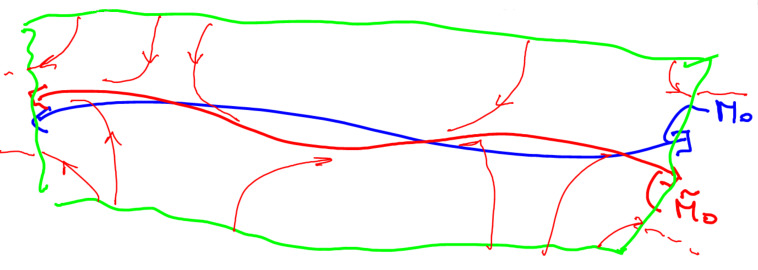
\includegraphics[width=0.7\textwidth]{figures/ch9/15fenichel_thm2.png}
	\caption{The manifolds $M_0$ and $\tilde{M}_{0}$ illustrated within the locally invariant manifold $W^{S}_{ \textrm{loc} }(\tilde{M}_{0})$ (green).}
	\label{fig:fenichel_thm2}
\end{figure}
\end{theorem}

\begin{remark}[]
	\begin{enumerate}
		\item If $M_0$ is compact, normally hyperbolic invariant (without boundary), then it attracts \underline{all} nearby trajectories ($M_0$ is an attractor that smoothly persists);
		\item The integer $r$ featured in the theorem is the minimum of $f \in \mathcal{C}^{r_1}$, $M_0 \in \mathcal{C}^{r_2}$, and $\sigma(p) < \frac{1}{r_3}$ with the integers $r_i \in \mathbb{Z}^{+}$;
		\item Similar results hold for inflowing invariant manifolds that repel nearby initial conditions ($M_0$ and $\tilde{M}_{0}$ are persistent repellers);
		\item The theory also extends to saddle-type invariant manifolds too, e.g. the unstable manifold of an overflowing invariant manifold.
	\end{enumerate}
	Assume the tangent bundle $\left.T\mathbb{R}^{n}\right|_{M_0}$ has an invariant splitting, i.e. $T_{p}\mathbb{R}^{n} = T_pM_0 \oplus N_{p}^{U}M_0 \oplus N_{p}^{S}M_0$, then there exists an additional Fenichel-type number for $N^{U}M_0$ and $W^{U}_{ \textrm{loc} (M_0)}$ is robust. This is shown in Fig. \ref{fig:fenichel_thm_rmks}.
		\begin{figure}[h!]
			\centering
			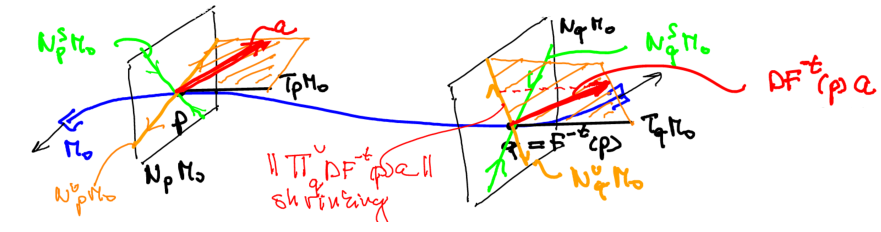
\includegraphics[width=0.7\textwidth]{figures/ch9/16fenichel_thm_rmks.png}
			\caption{The effect of the tangent bundle having an invariant splitting with the addition of a Fenichel-type number for $N^{U}M_0$ and robust $W^{U}_{ \textrm{loc} }(M_0)$.}
			\label{fig:fenichel_thm_rmks}
		\end{figure}
\end{remark}
For more see \cite{Wiggins1994}.

\section{Geometric singular perturbation theory}
